%% LyX 2.0.7.1 created this file.  For more info, see http://www.lyx.org/.
%% Do not edit unless you really know what you are doing.
\documentclass[english]{beamer}
\usepackage[T1]{fontenc}
\usepackage[latin9]{inputenc}
\usepackage{listings, fancyvrb}
\setcounter{secnumdepth}{3}
\setcounter{tocdepth}{3}
\setlength{\parindent}{0bp}

\makeatletter
%%%%%%%%%%%%%%%%%%%%%%%%%%%%%% Textclass specific LaTeX commands.
 % this default might be overridden by plain title style
 \newcommand\makebeamertitle{\frame{\maketitle}}%
 \AtBeginDocument{
   \let\origtableofcontents=\tableofcontents
   \def\tableofcontents{\@ifnextchar[{\origtableofcontents}{\gobbletableofcontents}}
   \def\gobbletableofcontents#1{\origtableofcontents}
 }
 \long\def\lyxframe#1{\@lyxframe#1\@lyxframestop}%
 \def\@lyxframe{\@ifnextchar<{\@@lyxframe}{\@@lyxframe<*>}}%
 \def\@@lyxframe<#1>{\@ifnextchar[{\@@@lyxframe<#1>}{\@@@lyxframe<#1>[]}}
 \def\@@@lyxframe<#1>[{\@ifnextchar<{\@@@@@lyxframe<#1>[}{\@@@@lyxframe<#1>[<*>][}}
 \def\@@@@@lyxframe<#1>[#2]{\@ifnextchar[{\@@@@lyxframe<#1>[#2]}{\@@@@lyxframe<#1>[#2][]}}
 \long\def\@@@@lyxframe<#1>[#2][#3]#4\@lyxframestop#5\lyxframeend{%
   \frame<#1>[#2][#3]{\frametitle{#4}#5}}
 \def\lyxframeend{} % In case there is a superfluous frame end

%%%%%%%%%%%%%%%%%%%%%%%%%%%%%% User specified LaTeX commands.
\usetheme[secheader]{Madrid}
\DeclareMathOperator*{\argmax}{arg\,max}
\makeatletter
\setbeamertemplate{footline}
{
  \leavevmode%
  \hbox{%
  \begin{beamercolorbox}[wd=.333333\paperwidth,ht=2.25ex,dp=1ex,center]{author in head/foot}%
    \usebeamerfont{author in head/foot}{Methods and Computing}
  \end{beamercolorbox}%
  \begin{beamercolorbox}[wd=.333333\paperwidth,ht=2.25ex,dp=1ex,center]{title in head/foot}%
    \usebeamerfont{title in head/foot}{Harvard University}
  \end{beamercolorbox}%
  \begin{beamercolorbox}[wd=.333333\paperwidth,ht=2.25ex,dp=1ex,right]{date in head/foot}%
    \usebeamerfont{date in head/foot}{Department of Biostatistics}
    \insertframenumber{} / \inserttotalframenumber\hspace*{2ex} 
  \end{beamercolorbox}}%
  \vskip0pt%
}
\makeatother

\makeatother

\usepackage{babel}
\begin{document}

\title{Biostatistics Preparatory Course:\\
Methods and Computing}


\author{Lecture 9}


\date{Maximum Likelihood \& the Bootstrap}

\makebeamertitle

\begin{frame}{Overview: Maximum Likelihood Estimation}
Consider estimating a parameter $\theta$ given a sample of data, $\{ X_1, \dots, X_n\}$

\vspace{7mm}
What is maximum likelihood estimation?
\begin{itemize}
	\item A statistical method that estimates $\theta$ as the value that maximizes the {\color{blue}likelihood} of obtaining the observed data
	\item That is, the maximum likelihood estimator ({\color{blue}MLE}) provides the greatest amount of agreement between the selected model and the data
\end{itemize}
\end{frame}


\begin{frame}{Overview: Maximum Likelihood Estimation}
\vspace{2mm}
What is the likelihood function?
\begin{itemize}
\item In math - $\mathcal{L}(\theta) = f(x_1, \dots, x_n | \theta)$ where $f(\cdot)$ denotes the joint density of the data
\item In words - the function that dictates the probability (relative frequency) of observing the data as a function of $\theta$ 
\end{itemize}

\vspace{5mm}
The definition of the MLE is:\\

\vspace*{2mm}\hspace*{1.5in}$ \hat{\theta}_{MLE} = \argmax_\theta \mathcal{L}(\theta)$
\end{frame}

\begin{frame}{Simple Setting}
We will focus on the setting of \emph{iid} observations, that is, \\
\begin{center}
$\{ X_1, \dots, X_n\} \quad \mbox{is a {\emph{simple random sample}}}$
\end{center}
\begin{itemize}
\item The likelihood then simplifies to 
$$\mathcal{L}(\theta) = \prod_{i = 1}^n f(x_i| \theta)$$
\item In practice, we typically maximize the log of the likelihood:
$$\ell(\theta) = \log\{\mathcal{L}(\theta)\} =  \sum_{i = 1}^n \log\{f(x_i| \theta)\}$$
since taking the derivative of a sum is typically easier than a product and the likelihood can be very small for large $n$   (a computational issue)
\end{itemize}
\end{frame}

\begin{frame}{Why is maximum likelihood estimation so popular?}
\begin{itemize}
\item Provides a unified framework for estimation
\item Under mild regularity conditions, MLEs are:
\begin{enumerate}
\item {\color{blue} consistent} $\rightarrow$ converge to the true value in probability as $n \to \infty$, i.e.
$$\lim_{n \to \infty} P(|\hat{\theta} - \theta | \le \epsilon)  = 1 \quad \forall \epsilon > 0 $$
\item {\color{blue} asymptotically normal} $\rightarrow$ $\sqrt{n}(\hat{\theta} - \theta) \sim N(0, \sigma^2)$ for large $n$
\item {\color{blue} asymptotically efficient} $\rightarrow$ achieve the lowest variance for large $n$
\item {\color{blue} invariant} $\rightarrow$ if $\hat{\theta}$ is the MLE for $\theta$ then $g(\hat{\theta})$ is the MLE for $g(\theta)$
\end{enumerate}
\item Many algorithms exist for maximum likelihood estimation
\end{itemize}
\end{frame}

\begin{frame}{Steps to find the MLE}
\begin{enumerate}
\item Write out the likelihood $$\mathcal{L}(\theta) = f(x_1, \dots, x_n | \theta)$$
\item Simplify the log likelihood $$\ell(\theta) = \log\{\mathcal{L}(\theta)\}$$
\item Take the derivative of $\ell(\theta)$ with respect to the parameter of interest, $\theta$
\item Set = 0
\item Solve for $\theta$ (this is your  $\hat{\theta}_{MLE}$)
\item Check that $\hat{\theta}_{MLE}$ is a maximum $\left(\frac{\partial^2}{\partial\theta^2}\ell(\theta)<0\right)$
\end{enumerate}
\end{frame}


\begin{frame}{MLE Exercises}
\pause 
\begin{enumerate}
	\item Suppose we have an iid sample $\{X_1, \dots, X_{100} \}$ with $X_i \sim Ber(p)$. Find the MLE for $p$. Recall that the density for a Bernoulli random variable can be written as: 
	
	$$ p^{X_i} (1-p)^{1-X_i} $$
	
	\vspace{3mm}
	\pause
	\item Suppose we have an iid sample $\{X_1, \dots, X_n \}$ with $X_i \sim N(\mu,\sigma^2)$ Find the MLE for $\mu$. Recall that the density for a normal random variable can be written as: 
	
	$$ \frac{1}{\sqrt{2\pi}\sigma} \exp( \frac{1}{2\sigma^2} (X_i - \mu)^2) $$
\end{enumerate}
\end{frame}

\begin{frame}{MLE Exercises in R}

We are going to use R to derive the MLE in more complex cases. 

\begin{itemize} 
	\item In the previous two examples, we found a closed-form solution (MLE) for our parameters
	\item Sometimes, there is no closed-form solution, so we need to use optimization methods to estimate our parameter of interest 
\end{itemize}

\end{frame}

\begin{frame}{The \tt{optim} function}

\begin{itemize}
	\item General-purpose optimization that implements various methods 
	\item It will find the values of some parameters that \textit{minimizes} some function 
	\item You need to specify...
	\begin{itemize}
		\item The parameters that you want to estimate 
		\item The function (in our case, the negative log-likelihood; why negative?)
		\item The method (I typically use "BFGS")
		\item Starting values for your parameters (use random numbers)
		\item Other values that you need to pass into your function
	\end{itemize}
\end{itemize}

\end{frame}

\begin{frame}{MLE Exercises}
\end{frame}


\begin{frame}{The Bootstrap}
\begin{itemize}
\item What is the bootstrap?
\begin{itemize}
\item A widely applicable, computer intensive resampling method used to compute standard errors, confidence intervals, and significance tests
\end{itemize}

\vspace{3mm}
\item Why is it important?
\begin{itemize}
\item The exact sampling distribution of an estimator can be difficult to obtain 
\item Asymptotic expansions are sometimes easier but expressions for standard errors based on large sample theory may not perform well in finite samples
\end{itemize}
\end{itemize}
\end{frame}



\begin{frame}{Motivating Analogy}
\centering

\includegraphics[scale = 0.4]{lecture7_2} \\


The bootstrap samples should relate to the original sample just as the original sample relates to the population
\end{frame}


\begin{frame}{Overview: The Bootstrap Principle}
\centering
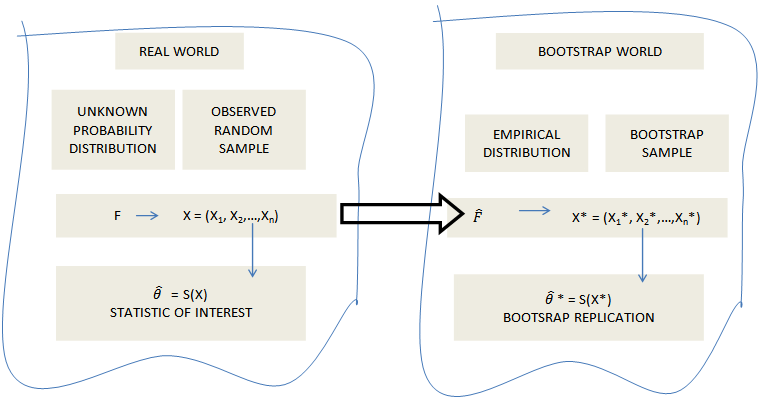
\includegraphics[scale = 0.4]{lecture7_1}

Without additional information, the sample contains all we know about the underlying distribution so resampling the sample is the best approximation to sampling from the true distribution 
\end{frame}

\begin{frame}{The Bootstrap Principle}
Suppose $X = \{X_1, \dots, X_n\}$ is a sample used to estimate some parameter $\theta = T(P)$ of the underlying distribution $P$.  To make inference on $\theta$, we are interested in the properties of our estimator $\hat{\theta} = S(X)$ for $\theta$.

\vspace{3mm}
\begin{itemize}
\item If we knew $P$, we could obtain $\{X^b | b = 1, \dots B\}$ from $P$ and use Monte-Carlo to estimate the sampling distribution of $\hat{\theta}$ (sound familiar?)
\item We don't so we do the next best thing and resample from original sample, i.e. {\emph{the empirical distribution, $\hat{P}$}} 
\begin{itemize}
\item We expect the empirical distribution to estimate the underlying distribution well by the {\emph{Glivenko-Cantelli Theorem}}
\end{itemize}
\end{itemize}
\end{frame}

\begin{frame}{Bootstrap procedure}
Goal: Find the standard error and confidence intervals for some $\hat{\theta} = S(\mathbf{D})$ where $\mathbf{D}$ encodes our observed data.

\begin{itemize}
	\item Select $B$ independent bootstrap resamples $\mathbf{D}(b)$, each consisting of $N$ data values drawn with replacement from the data.
	\item Compute the estimates from each bootstrap resample
	$$\hat{\theta}^*(b) = S(\mathbf{D}^*(b))\ \ b=1,...,B$$
	\item Estimate the standard error $se(\hat{\theta})$ by the sample standard deviation of the $B$ replications of $\hat{\theta}^*(b)$
	\item Estimate the confidence interval by finding the $100(1-\alpha)$ percentile bootstrap CI, 
	$$(\hat{\theta}_L, \hat{\theta}_U) = (\hat{\theta^*}^{\alpha/2}, \hat{\theta^*}^{1-\alpha/2}) $$
\end{itemize}
\end{frame}


\begin{frame}{Boostrap exercise}
\end{frame}

\end{document}


\begin{frame}{Example: The Median}
The distribution of the sample median $\hat{m}$ is asymptotically normal with mean $m$ and variance
$$\frac{1}{4nf^2(m)}$$
where $m$ is the median of the data generating distribution $f(x)$ and $n$ is the sample size.

\vspace{3mm}
Run a simulation with 500 trials to see how well the bootstrap approximates the variance of the median for samples of size 100 from a $N(3, 2)$.  What would be an appropriate number of bootstrap replicates? Summarize your results.
\end{frame}
